\documentclass[a4paper,11pt]{article}

\usepackage{minted}

% Package to make citations superscrit with brackets
%\usepackage[super,square]{natbib}

% Package to change margin size
\usepackage{anysize}
\marginsize{2cm}{2cm}{1cm}{2cm}
% Package to make headers
\usepackage{fancyhdr}
\setlength{\headheight}{13.6pt} % Fix for fancyhdr warning
\renewcommand{\headrulewidth}{0pt}
% Package for highligths
\usepackage{soul}
% Colors for the references links
\usepackage[dvipsnames]{xcolor}
% Package to link references
\usepackage{hyperref}
\hypersetup{
    colorlinks=true,
    linkcolor=blue,
    citecolor=blue,
    filecolor=blue,      
    urlcolor=blue,
}
% Package for lorem ipsum
\usepackage{lipsum}
% Package for multicolumn
\usepackage{multicol}
% Package for removing paragraph identations
\usepackage{parskip}
\setlength\columnsep{18pt}
% Sets abstract
\renewenvironment{abstract}
 {\par\noindent\textbf{\abstractname}\ \ignorespaces\\}
 {\par\noindent\medskip}

\usepackage{graphicx}

\usepackage{amsmath}

\usepackage{caption}

\usepackage{amssymb}

\usepackage{tikz}

\usepackage{float}

\usepackage{listings}

\begin{document}

\begin{titlepage}
    \pagestyle{empty}
    \begin{center}
        % Logo
        
\includegraphics[width=0.25\textwidth]{isologo-utec.png} % Adjust path/size as needed
        \vspace{1cm}

        % Title
        {\LARGE\textbf{Laboratorio 14}}
        \vspace{1.5cm}

        % Authors
        {\large
            \textbf{Integrantes:} \\
            Casquino, Daniel: 202110056 \\
            Niño, Jesús: 202310452 \\
        }
        \vspace{1cm}

        % Course
        {\large
            \textbf{Curso:} Base de Datos II --- (CS2042)
        }
        \vspace{0.5cm}

        % Teacher
        {\large
            \textbf{Docente:} Heider Sanchez
        }
        \vspace{0.5cm}

        % Date
        {\large
            \textbf{Fecha de presentación:} 01 de Julio de 2025
        }
        \vfill

        {\large
            Universidad de Ingeniería y Tecnología (UTEC)
        }
    \end{center}
\end{titlepage}

% Makes header
\pagestyle{fancy}
\thispagestyle{empty}
\fancyhead[R]{\textit{Universidad de Ingeniería y Tecnología --- UTEC}}
\fancyhead[L]{}
% Makes footnotes with an asterisk
\renewcommand*{\thefootnote}{\fnsymbol{footnote}}


\medskip
\section{P1: Gestión de Productos y Pedidos}

\subsection{Colecciones y Datos}

Primero, se crearon las~\hyperref[fig:collections]{colecciones}:

\begin{minted}{javascript}
use lab13
db.createCollection("Productos")
db.createCollection("Clientes")
db.createCollection("Pedidos")
\end{minted}

Luego, se insertaron los datos de los archivos json desde \hyperref[fig:clientes]{MongoDB Compass}. Además,
se generaron datos adicionales con ChatGPT para evaluar mejor las consultas.

\subsection{Consultas}

Los resultados de estas consultas se pueden ver en la sección de \hyperref[consultas]{consultas} del anexo.

$\bullet$ \textbf{Obtener todos los clientes de Chile:} Esta consulta filtra los documentos por el subcampo \textit{país}
del campo \textit{dirección}.
\begin{minted}{javascript}
db.clientes.find({"direccion.pais": "Chile"})
\end{minted}

$\bullet$ \textbf{Obtener los pedidos de un cliente específico (por ID):} Similar a la consulta anterior, se hace
un filtrado por el campo \textit{id$\_$cliente} de los pedidos.
\begin{minted}{javascript}
db.pedidos.find({"id_cliente": 1})
\end{minted}

$\bullet$ \textbf{Obtener los pedidos con un total superior a cierto valor:} El filtrado se realiza en el campo
\textit{total$\_$pedido}, y seleccionamos los atributos más relevantes.
\begin{minted}{javascript}
db.pedidos.find(
    {"total_pedido": {$gt: 800}},
    {"id_cliente": 1, "id_pedido": 1, "total_pedido": 1, "_id": 0}
)
\end{minted}

$\bullet$ \textbf{Contar el número total de pedidos entre un rango de fechas:} Primero, realizamos un \textit{match} para seleccionar
los pedidos que cumplen con el criterio de fecha, y usamos \textit{count} para contar la cantidad de pedidos que cumplen la condicion.
\begin{minted}{javascript}
db.pedidos.aggregate([
    {$match:{"fecha_pedido": {$gte: "2024-09-17", $lt: "2024-09-22"}}},
    {$count: "total"}
])
\end{minted}

$\bullet$ \textbf{¿Cuáles son los $k$ productos más vendidos?} En esta consulta, usamos \textit{unwind} para desglosar los arreglos
de productos de cada pedido. Luego, los agrupamos por \textit{id$\_$producto}, y hallamos el total usando \textit{sum}. Para filtrar los
$k$ productos más vendidos, ordenamos por cantidad y limitamos el output.
\begin{minted}{javascript}
db.pedidos.aggregate([
    {$unwind: "$productos"},
    {$group: {
            _id: "$productos.id_producto",
            cantidad: {$sum: "$productos.cantidad"}
        }
    },
    {$sort: {"cantidad": -1}},
    {$limit: 5}
])
\end{minted}

Nota: En este ejemplo, obtenemos los 5 productos más vendidos. Podemos
reemplazar el 5 por cualquier otro número.

$\bullet$ \textbf{¿Quiénes son los clientes más frecuentes?} Para la consulta, agrupamos los pedidos por el id del cliente,
y hacemos la sumatoria de la cantidad de pedidos. Finalmente, ordenamos por cantidad de pedidos y limitamos el output.
\begin{minted}{javascript}
db.pedidos.aggregate([
    {$group: {
        _id: "$id_cliente",
        n_pedidos: {$sum: 1}
        }
    },
    {$sort: {"n_pedidos": -1}},
    {$limit: 5}
])
\end{minted}

Nota: En este ejemplo, obtenemos los 5 clientes más frecuentes.

\subsection{Reto Adicional}

Para crear los \hyperref[fig:creacionindices]{índices} en los campos \texttt{fecha\_pedido} y \texttt{id\_cliente}, usamos
las siguientes consultas:

\begin{minted}{javascript}
db.pedidos.createIndex({ fecha_pedido: 1 })
db.pedidos.createIndex({ id_cliente: 1 })
\end{minted}

Para utilizar el primer índice, podemos realizar una búsqueda de pedidos en un rango de fechas:

\begin{minted}{javascript}
db.pedidos.find({
    "fecha_pedido": { $gte: "2024-09-15", $lt: "2024-09-21" }
})
\end{minted}

Y para el segundo índice, buscar los pedidos realizados por un cliente en particular:

\begin{minted}{javascript}
db.pedidos.find({
    "id_cliente": 3
})
\end{minted}
\section{P2: Gestión de Productos con Python}

\subsection{Carga con API Pública}

Primero, completamos la función de \textit{fetching} de datos.

\begin{minted}{python}
def fetch_all_categories(self, base_url):
    # cada objeto en base_url tiene:
    # slug, name, url
    response = self.fetch_json_data(base_url)
    self.db.categorias.insert_many(response)
\end{minted}

Con esta función, obtenemos todas las categorías de productos desde la API, y las
insertamos en la colección \texttt{categorias} en Mongo.

Luego, completamos la función de obtención de productos.

\begin{minted}{python}
def fetch_all_products(self):
documents = self.db.categorias.find()
for doc in documents:
    response = self.fetch_json_data(doc["url"])
    print(f"Fetched {len(response["products"])} items for category {doc["name"]}")
    self.db.productos.insert_many(response["products"])
\end{minted}

Después, probamos la conexión a nuestro Atlas cluster, reemplazando el URI por el \textit{connection string}
que nos da el app web.

\begin{figure}[H]
    \centering
    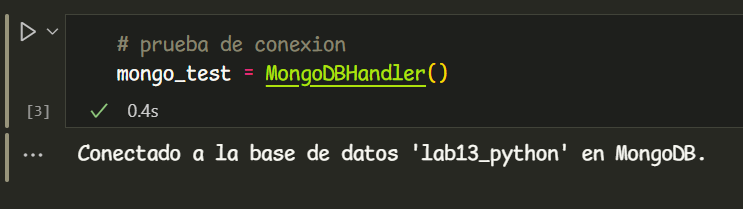
\includegraphics[width=0.6\textwidth]{./p2_pruebaconexion.png}
    \caption{Conexión a MongoDB desde Python}\label{fig:pruebaconexion}
\end{figure}

Luego, encapsulamos la funcionalidad de \textit{fetching} en una función, la cual sólo se
ejecuta una vez para cargar los datos a nuestro cluster.

\begin{figure}[H]
    \centering
    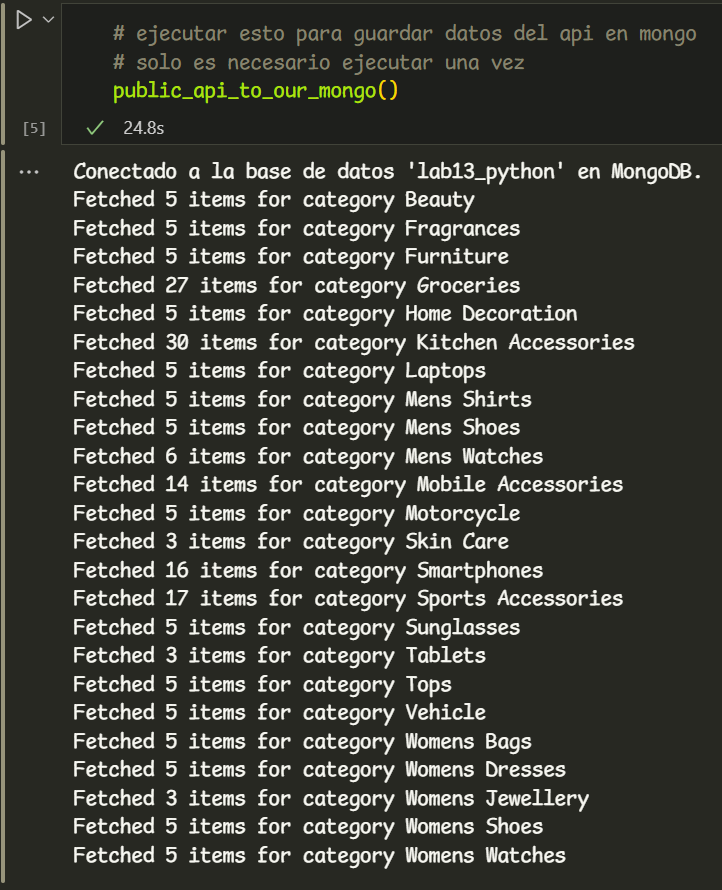
\includegraphics[width=0.6\textwidth]{./p2_fetching.png}
    \caption{Fetching de datos}\label{fig:fetching}
\end{figure}

Luego de ejecutar la función, podemos ver que los datos \hyperref[cargadatos]{se han cargado correctamente}.

\subsection{CRUD y Filtrado}

Luego de cargar los datos a Mongo, implementamos las funciones de CRUD y filtrado que se solicitaron.

\begin{figure}[H]
    \centering
    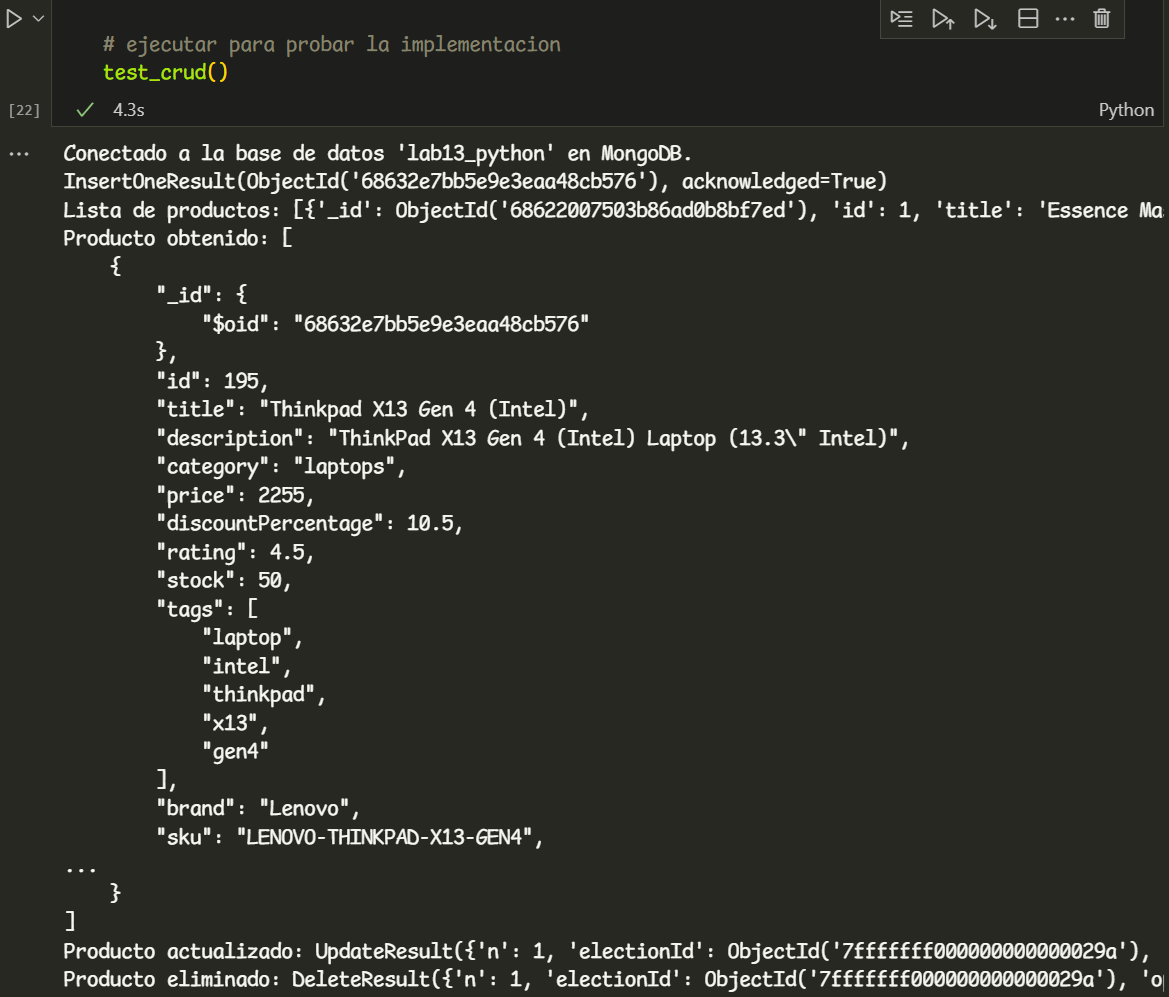
\includegraphics[width=0.6\textwidth]{./p2_crud.png}
    \caption{CRUD desde Python}\label{fig:crud}
\end{figure}

Finalmente, ejecutamos las funciones de agregación. Los resultados se muestran a continuación:

\begin{figure}[H]
    \centering
    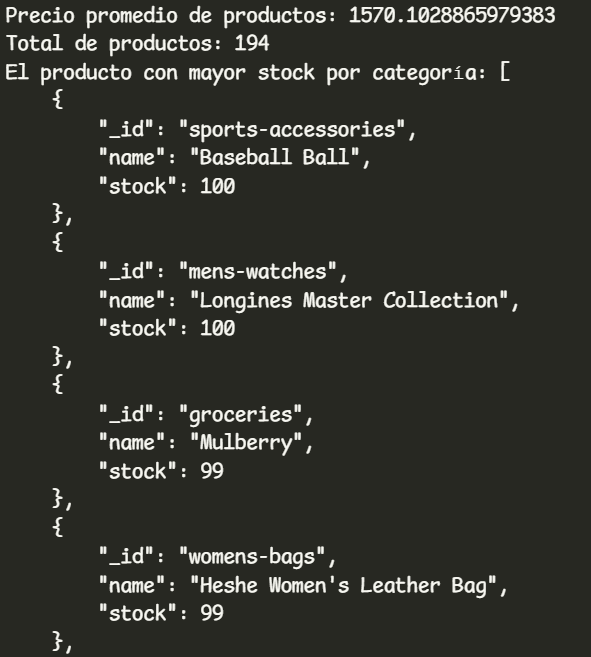
\includegraphics[width=0.4\textwidth]{./p2_agregadas.png}
    \caption{Resultado de promedio, total y máximo de productos por categoría}\label{fig:agregadas}
\end{figure}

Nota: El \textit{notebook} con la implementación de la clase \textbf{MongoDBHandler} se encuentra en el repositorio de \hyperref[repo]{GitHub} disponible
en el anexo.

\newpage

\appendix
\section{Anexo}

\subsection{Configuración de Sharding}
\begin{figure}[H]
    \centering
    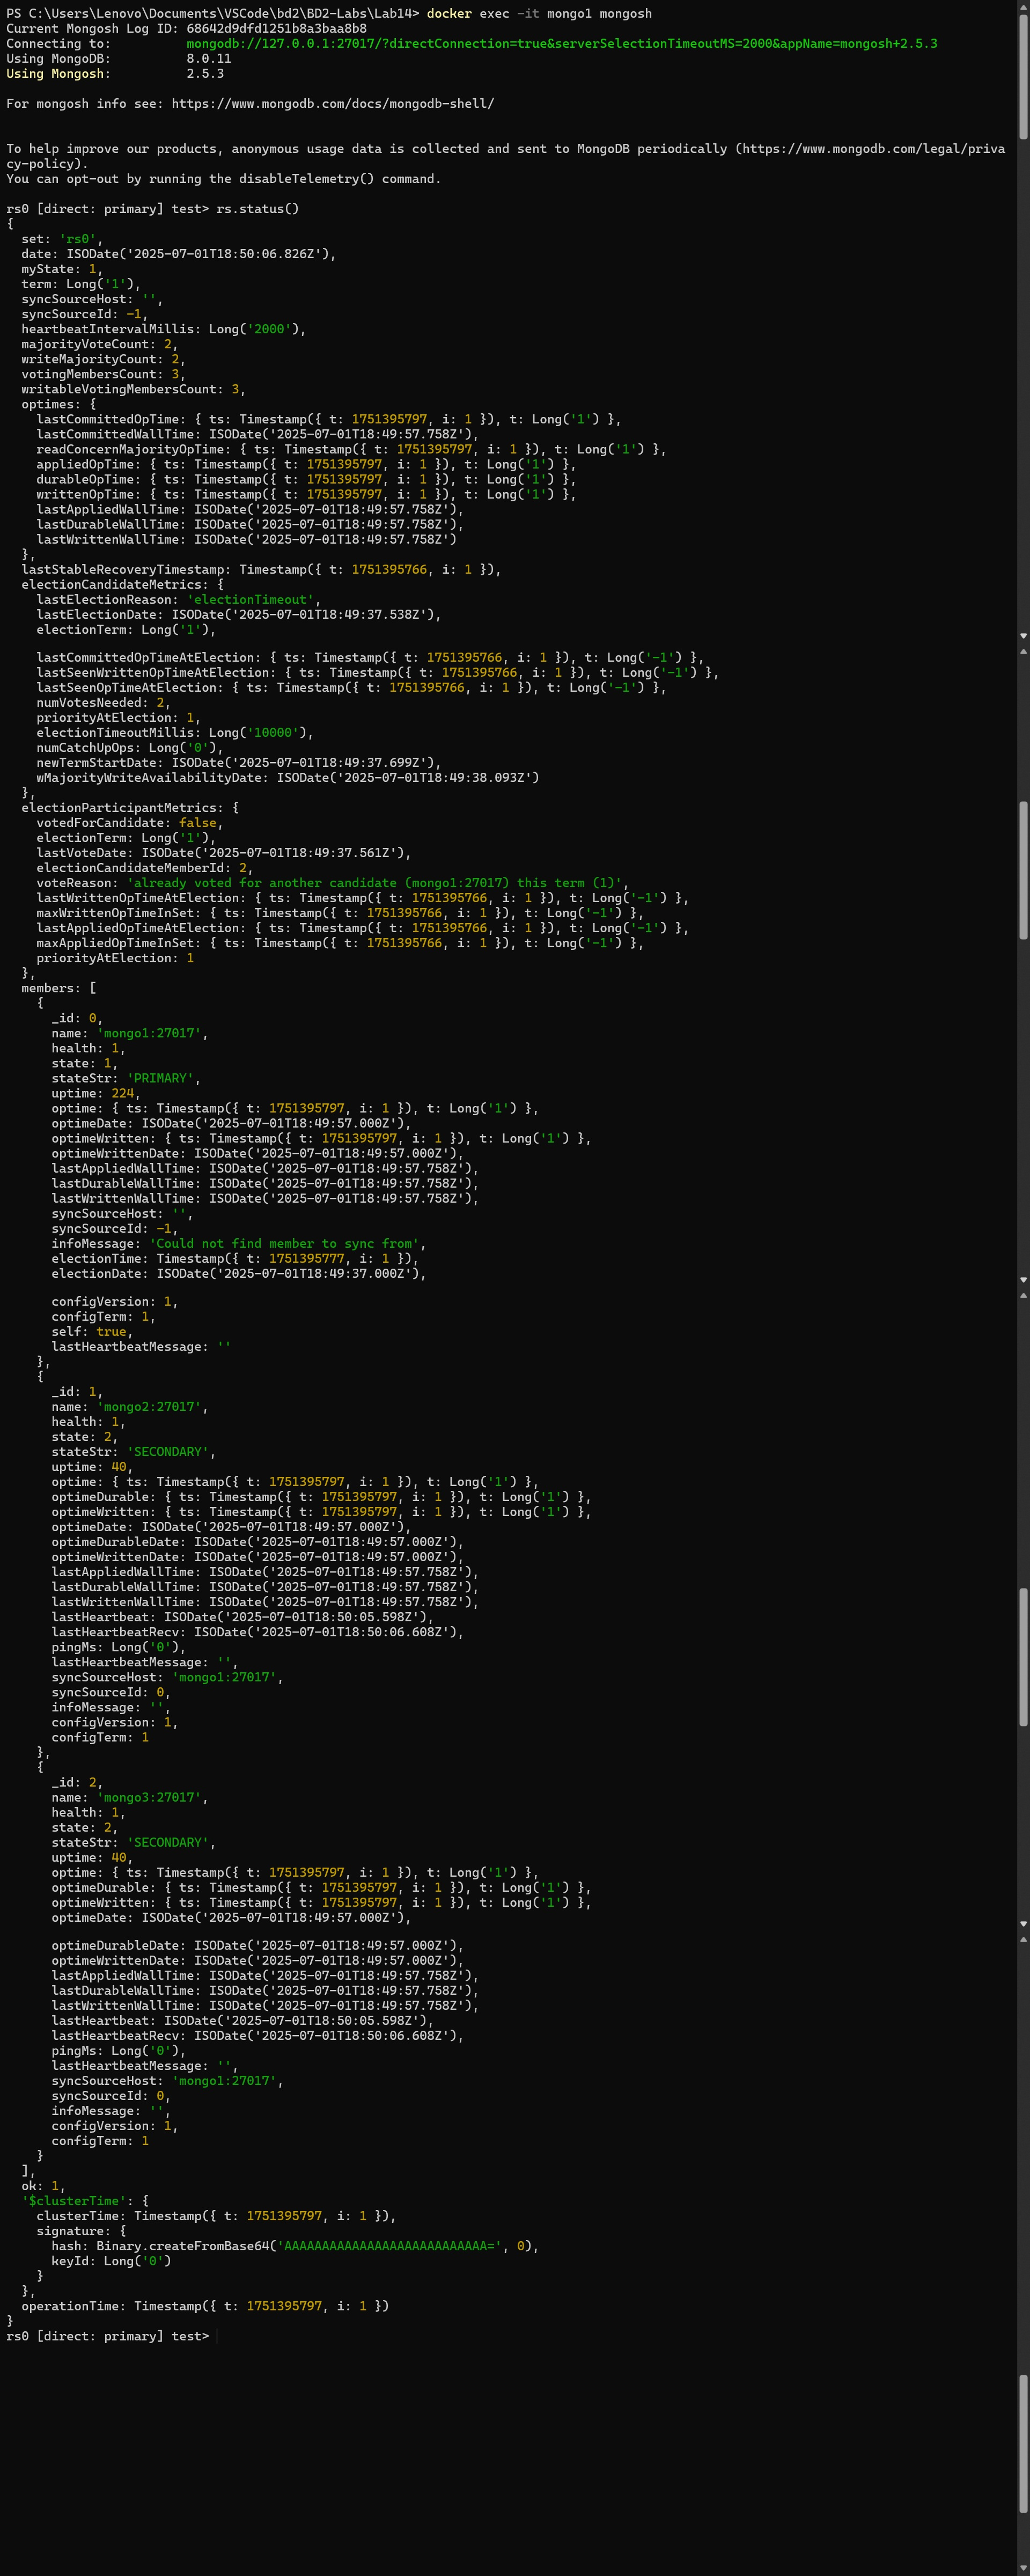
\includegraphics[width=0.5\textwidth]{./sharding.jpg}
    \caption{Resultado de rs.status ()}\label{fig:sharding}
\end{figure}

\subsection{Búsqueda de Texto}

\subsubsection{Inserción de Datos}\label{insercion}

\begin{figure}[H]
    \centering
    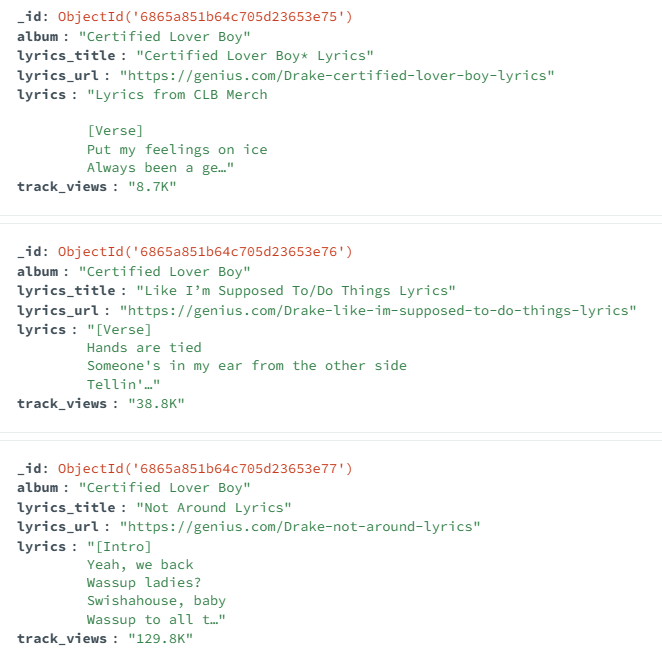
\includegraphics[width=0.6\textwidth]{./insercion_drake.png}
    \caption{Canciones de Drake en MongoDB Compass}\label{fig:inserciondrake}
\end{figure}

\begin{figure}[H]
    \centering
    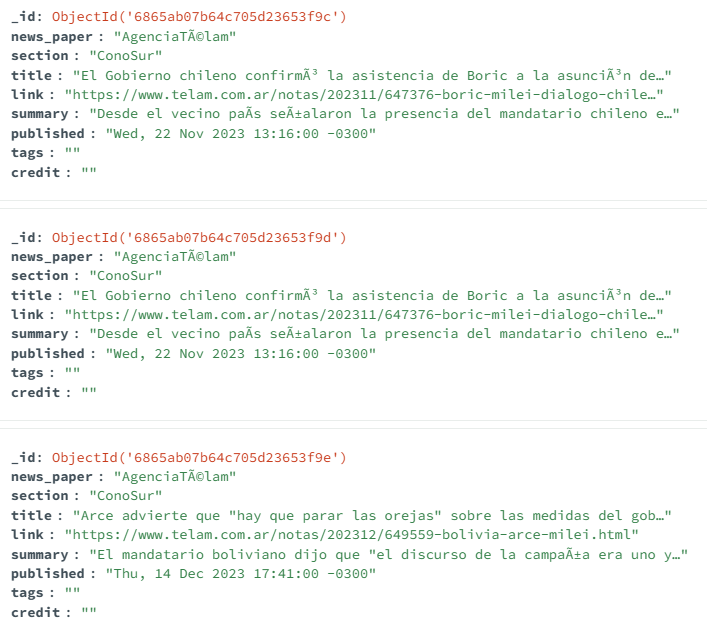
\includegraphics[width=0.6\textwidth]{./insercion_milei.png}
    \caption{Artículos sobre Milei en MongoDB Compass}\label{fig:insercionmilei}
\end{figure}

\end{document}